\documentclass{cumcmthesis}

\usepackage{tikz}
\usetikzlibrary{arrows.meta}
\usetikzlibrary{patterns}
\usepackage{pgfplots}

\pgfplotsset{compat = 1.8}
\pgfplotsset{every axis label/.append style={font=\small}}
\pgfplotsset{every tick label/.append style={font=\small}}
\pgfplotsset{every legend label/.append style = {font = \small}}

\newcommand{\prb}{\times 10^5~\mathrm{kPa}}
\newcommand{\pre}{~\mathrm{kPa}}
\newcommand{\vol}{~\mathrm{mm^3}}
\newcommand{\are}{~\mathrm{mm^2}}
\newcommand{\len}{~\mathrm{mm}}
\newcommand{\tim}{~\mathrm{ms}}
\newcommand{\vel}{~\mathrm{ms^{-1}}}
\newcommand{\mas}{~\mathrm{mg}}
\newcommand{\den}{~\mathrm{mg~mm^{-3}}}
\newcommand{\flo}{~\mathrm{mm^3~ms^{-1}}}

\newcommand{\pres}{/\mathrm{kPa}}
\newcommand{\vols}{/\mathrm{mm^3}}
\newcommand{\ares}{/\mathrm{mm^2}}
\newcommand{\lens}{/\mathrm{mm}}
\newcommand{\tims}{/\mathrm{ms}}
\newcommand{\vels}{/\mathrm{ms^{-1}}}
\newcommand{\mass}{/\mathrm{mg}}
\newcommand{\dens}{/\mathrm{mg~mm^{-3}}}
\newcommand{\flos}{/\mathrm{mm^3~ms^{-1}}}
\usepackage{listings}
\usepackage{xcolor}
\usepackage{lmodern}
% 配置代码高亮
\lstset{
	basicstyle          =   \sffamily,          % 基本代码风格
	keywordstyle        =   \bfseries,          % 关键字风格
	commentstyle        =   \rmfamily\itshape,  % 注释的风格,斜体
	stringstyle         =   \ttfamily,  % 字符串风格
	flexiblecolumns,                % 别问为什么,加上这个
	numbers             =   left,   % 行号的位置在左边
	showspaces          =   false,  % 是否显示空格,显示了有点乱,所以不现实了
	numberstyle         =   \zihao{-5}\ttfamily,    % 行号的样式,小五号,tt等宽字体
	showstringspaces    =   false,
	captionpos          =   t,      % 这段代码的名字所呈现的位置,t指的是top上面
	frame               =   lrtb,   % 显示边框
}
\lstdefinestyle{Python}{
	language        =   Python, % 语言选Python
	basicstyle      =   \zihao{-5}\ttfamily,
	numberstyle     =   \zihao{-5}\ttfamily,
	keywordstyle    =   \color{blue},
	keywordstyle    =   [2] \color{teal},
	stringstyle     =   \color{magenta},
	commentstyle    =   \color{red}\ttfamily,
	breaklines      =   true,   % 自动换行,建议不要写太长的行
	columns         =   fixed,  % 如果不加这一句,字间距就不固定,很丑,必须加
	basewidth       =   0.5em,
}
\begin{document}

\begin{thebibliography}{9}%宽度9
	\bibitem[1]{引言}
    白云.
    \newblock 高压共轨燃油系统循环喷油量波动特性研究\allowbreak[D].
    \newblock 哈尔滨工程大学,2017.

	\bibitem[2]{保持频率不变}
    仲志全,李华宇,尹琪.
    \newblock 发动机运行工况对机油耗影响的试验研究\allowbreak[J].
    \newblock 内燃机工程,2004(05):69-71.

	\bibitem[3]{减压阀}
    刘学龙,苏万华,战强.
    \newblock 高压油管对共轨系统性能影响的研究\allowbreak[J].
    \newblock 内燃机工程,2010,31(05):47-51+57.

	\bibitem[4]{锥形喷油嘴}
    陶希成.
    \newblock 柴油机锥形孔喷嘴内空穴流动及其对喷雾影响的试验研究\allowbreak[D].
    \newblock 江苏大学,2016.

    \bibitem[5]{模型评价1}
    崔慧峰,罗福强,董少锋,梁昱,周立迎.
    \newblock 柴油机渐缩形喷孔喷嘴流动特性研究\allowbreak[J].
    \newblock 农业机械学报,2013,44(11):19-25.

    \bibitem[6] {模型评价2}
    丁晓亮,张幽彤,苏海峰. 
    \newblock 压电式共轨系统喷油量压力波动修正策略研究\allowbreak[J].
    \newblock 北京理工大学学报. 2010(09)
\end{thebibliography}

\section{引言}
高压油管被广泛应用于柴油机等燃油发动机中,燃油经过高压油泵进入高压油管,
再由喷口喷出。燃油的周期性进入与喷出会导致高压油管内压力的变化,直接影响其所匹配燃油机性能的稳定性和工作
的可靠性。具体而言,管内压强的波动将导致排气温度不稳定,降低了催化剂的转换效
率,使燃油机排放一致性下降。因此,减小管内压力的波动从而提升工作效率,是当前高压燃油系统亟需
解决的技术难题。






\begin{figure}[!ht]
	\centering
	\begin{tikzpicture}
	\begin{axis} [
		width = 10cm,
		height = 5cm,
		xlabel = {$t\tims$},
		ylabel = {$P_2-P_2^*\pres$},
		xmin = 0, 
		xmax = 500,
		ymin = -200,
		ymax = 200,
		%ytick distance = 400,
	]
	\addplot table [
		x=t, 
		y=P_2, 
		mark=none, 
		smooth] {../3/t-P-1.dat};
	\end{axis}
	\end{tikzpicture}
	\caption{$\tau_A=0.288\tim$ 时,油管在第一个周期内的压强随时间的变化关系}
	\label{firstperiodPt}
\end{figure}


\begin{figure}[!ht]
	\centering
	\begin{tikzpicture}
	\begin{axis} [
		width = 10cm,
		height = 5cm,
		xlabel = {$t\tims$},
		ylabel = {$P_2-P_2^*\pres$},
		xmin = 0, 
		xmax = 300,
		%ymin = -2400,
		%ymax = 400,
		%ytick distance = 400,
	]
	\addplot table [
		x=t, 
		y=P_2, 
		mark=none, 
		smooth] {../3/t-P-2.dat};
	\end{axis}
	\end{tikzpicture}
	\caption{$\tau_A=0.288\tim$ 时,油管在第一个周期内的压强随时间的变化关系}
	\label{firstperiodPt}
\end{figure}








\begin{figure}[!ht]
	\centering
	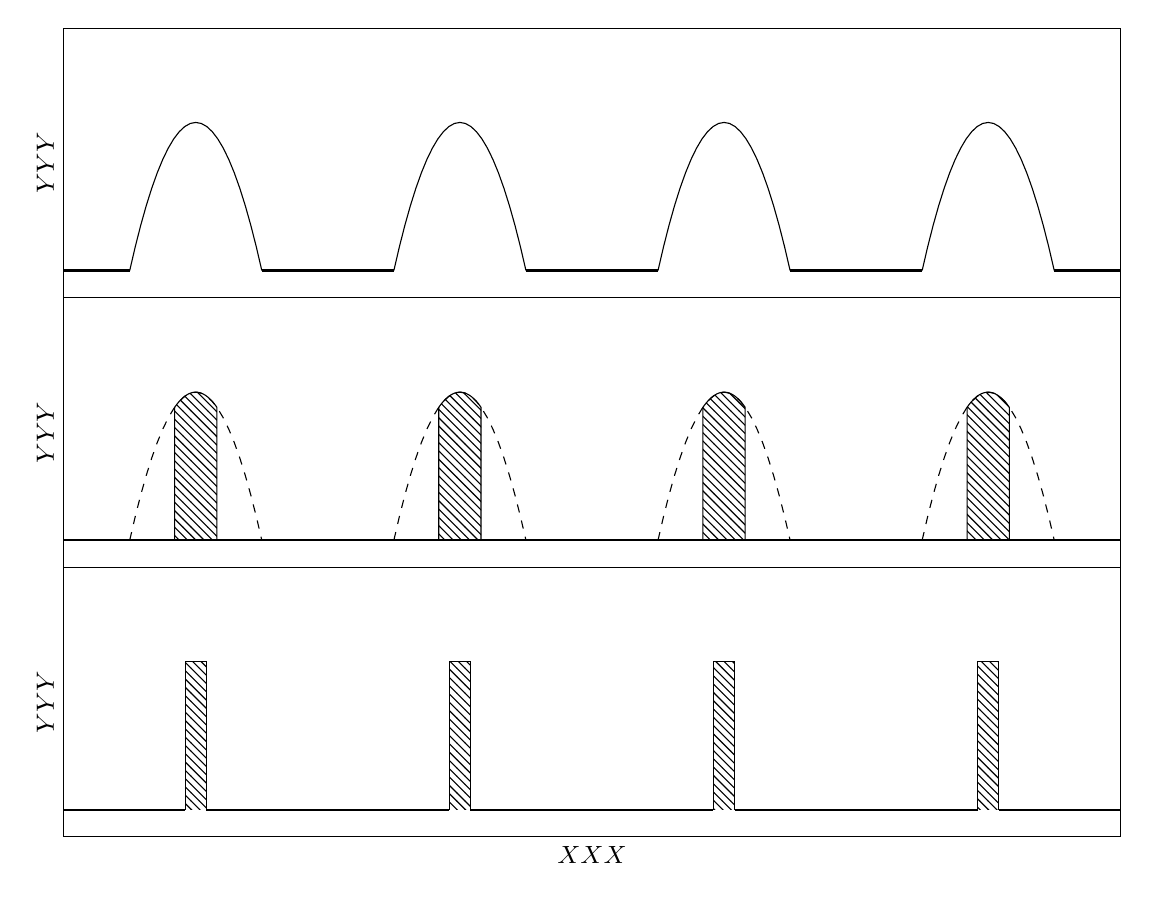
\begin{tikzpicture}
		\begin{axis}[
			name = first plot,
			xticklabel style = {
				color = white,
			},
			ylabel = {$YYY$},
			xmin = 0,
			xmax = 1000,
			ymin = 0,
			ymax = 100,
			width = 15cm,
			height = 5cm,
			xtick=\empty,
			ytick=\empty,
		]
		\draw[thick] (0,10) -- (6.25,10);
		\draw[domain=6.25:18.75] plot(\x,{-1.408*(\x-12.5)^2+65});
		\draw[thick] (18.75,10) -- (31.25,10);
		\draw[domain=31.25:43.75] plot(\x,{-1.408*(\x-37.5)^2+65});
		\draw[thick] (43.75,10) -- (56.25,10);
		\draw[domain=56.25:68.75] plot(\x,{-1.408*(\x-62.5)^2+65});
		\draw[thick] (68.75,10) -- (81.25,10);
		\draw[domain=81.25:93.75] plot(\x,{-1.408*(\x-87.5)^2+65});
		\draw[thick] (93.75,10) -- (100,10);
		\end{axis}





		\begin{axis}[
			name = second plot,
			at={(first plot.below south west)},
			yshift = 0cm,
			anchor = north west,
			xticklabel style = {
				color = white,
			xtick=\empty,
			ytick=\empty,
			},
			ylabel={$YYY$},
			xmin = 0,
			xmax = 1000,
			ymin = 0,
			ymax = 100,
			%ytick distance = 400,
			width = 15cm,
			height = 5cm,
		]
		\draw[thick] (0,10) -- (100,10);
		\draw[dashed,domain=6.25:18.75] plot(\x,{-1.408*(\x-12.5)^2+65});
		%\draw[thick] (18.75,10) -- (31.25,10);
		\draw[dashed,domain=31.25:43.75] plot(\x,{-1.408*(\x-37.5)^2+65});
		%\draw[thick] (43.75,10) -- (56.25,10);
		\draw[dashed,domain=56.25:68.75] plot(\x,{-1.408*(\x-62.5)^2+65});
		%\draw[thick] (68.75,10) -- (81.25,10);
		\draw[dashed,domain=81.25:93.75] plot(\x,{-1.408*(\x-87.5)^2+65});
		%\draw[thick] (93.75,10) -- (100,10);
		\draw[pattern=north west lines] (10.5,10) -- (10.5,59.368) plot [domain=10.5:14.5,smooth] (\x,{-1.408*(\x-12.5)^2+65})  -- (14.5,10) -- (10.5,10);
		\draw[pattern=north west lines] (35.5,10) -- (35.5,59.368) plot [domain=35.5:39.5,smooth] (\x,{-1.408*(\x-37.5)^2+65})  -- (39.5,10) -- (35.5,10);
		\draw[pattern=north west lines] (60.5,10) -- (60.5,59.368) plot [domain=60.5:64.5,smooth] (\x,{-1.408*(\x-62.5)^2+65})  -- (64.5,10) -- (60.5,10);
		\draw[pattern=north west lines] (85.5,10) -- (85.5,59.368) plot [domain=85.5:89.5,smooth] (\x,{-1.408*(\x-87.5)^2+65})  -- (89.5,10) -- (85.5,10);
		\end{axis}




		\begin{axis}[
			name = third plot,
			at={(second plot.below south west)},
			yshift = 0cm,
			anchor=north west,
			xlabel={$XXX$},
			ylabel={$YYY$},
			xmin = 0,
			xmax = 1000,
			ymin=0,
			ymax=100,
			width = 15cm,
			height = 5cm,
			xtick=\empty,
			ytick=\empty,
		]
		\draw[thick] (0,10) -- (11.5,10);
		\draw[thick] (13.5,10) -- (36.5,10);
		\draw[thick] (38.5,10) -- (61.5,10);
		\draw[thick] (63.5,10) -- (86.5,10);
		\draw[thick] (88.5,10) -- (100,10);
		\draw[pattern=north west lines] (11.5,10) -- (11.5,65) -- (13.5,65) -- (13.5,10);
		\draw[pattern=north west lines] (36.5,10) -- (36.5,65) -- (38.5,65) -- (38.5,10);
		\draw[pattern=north west lines] (61.5,10) -- (61.5,65) -- (63.5,65) -- (63.5,10);
		\draw[pattern=north west lines] (86.5,10) -- (86.5,65) -- (88.5,65) -- (88.5,10);
		\end{axis}



	\end{tikzpicture}
	\caption{题3用图}
\end{figure}


\begin{figure}
	\centering
	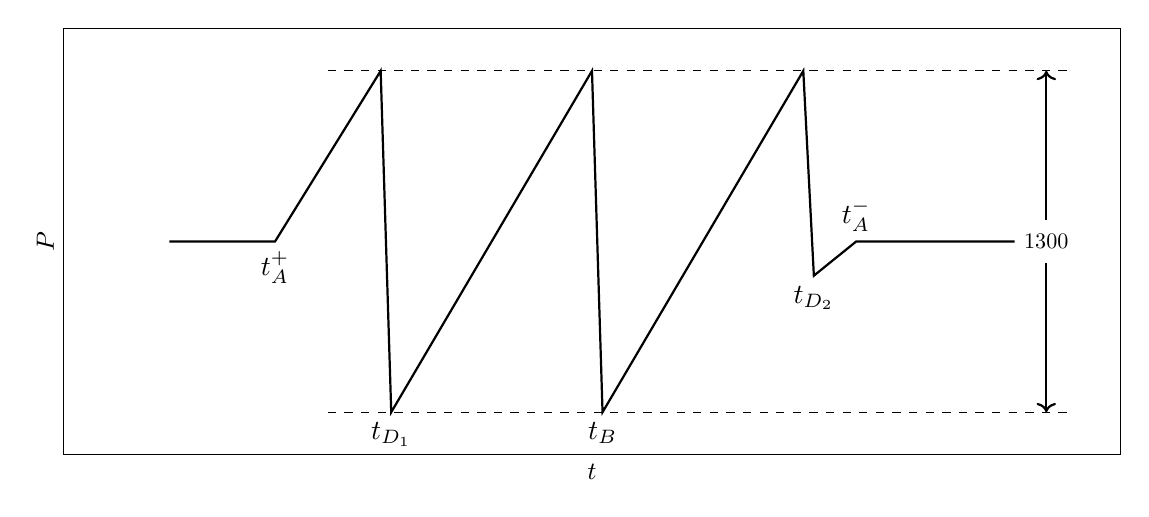
\begin{tikzpicture}
	\begin{axis}[
	width=15cm,
	height=7cm,
	xlabel=$t$,
	ylabel=$P$,
	xmin=0,
	xmax=1000,
	ymin=0,
	ymax=100,
	xtick=\empty,
	ytick=\empty,
	]
	\draw[thick] (10,50) -- (20,50) node[below,scale=1] {$t_A^+$}-- (30,90) -- (31,10)  node[below,scale=1] {$t_{D_1}$} -- (50,90) -- (51,10)  node[below,scale=1] {$t_B$} -- (70,90) -- (71,42)  node[below,scale=1] {$t_{D_2}$} -- (75,50)  node[above,scale=1] {$t_A^-$} -- (90,50);
	\draw[style=dashed] (25,90) -- (95,90);
	\draw[style=dashed] (25,10) -- (95,10);
	\draw[->,thick] (93,55) -- (93,90);
	\node [scale=0.8] at (93,50) {$1300$};
	\draw[->,thick] (93,45) -- (93,10) ;
	\end{axis}
	\end{tikzpicture}
	\caption{第三题用图}
	\label{tauN}
\end{figure}












































\end{document}